\chapter{Associatieve Geheugens}
\begin{itemize}
    \item Klassiek computergeheugen:
    \begin{itemize}
        \item Geef een adres op en krijg de inhoud op die geheugenplaats.
        \alert Dit adres moet correct zijn, of verkeerde inhoud wordt teruggegeven.
    \end{itemize}
    \item Associatief geheugen:
    \begin{itemize}
        \item Geef een gedeelte van de inhoud op en krijg daarmee de geassocieerde volledige inhoud terug.
        \item Speelt bij de mens een belangrijkere rol. 
    \end{itemize}

\end{itemize}
\section{Hopfieldnetten}
\begin{itemize}
    \item Een model voor een biologisch associatief geheugen.
    \item Eenvoudigste vorm = binaire patronen opslaan.
    \item De neuronen in een Hopfieldnet zijn dan ook TLU's met drempelwaarde nul.
    \item Alle neuronen zijn met alle andere neuronen verbonden, behalve zichzelf en de gewichten zijn symmetrisch:

    $$w_{ij} = w_{ji} \; \hbox{en} \; w_{ii} = 0$$
    \alert Geen aparte in- en uitvoerneuronen.
    \item Veronderstelling van bitpatroon dat evenveel bits heeft als neuronen in het netwerk.
    \item Elk neuron wordt in een toestand gebracht waarin het als uitvoer de overeenkomstige bitwaarde heeft.
    \item Sommige neuronen worden aangeduid voor herberekening, tot dat een stabiele toestand bereikt wordt (de geassocieerde eindtoestand).
    \item \underline{Voorbeeld}:
    \begin{itemize}
        \item Drie neuronen $x_1, x_2$ en $x_3$ met gewichtenmatrix
        $$W = \begin{pmatrix}
            0 & 1 & -2 \\
            1 & 0 & -2 \\
            -2 & -2 & 0
        \end{pmatrix}$$
        \begin{figure}[ht]
            \centering
            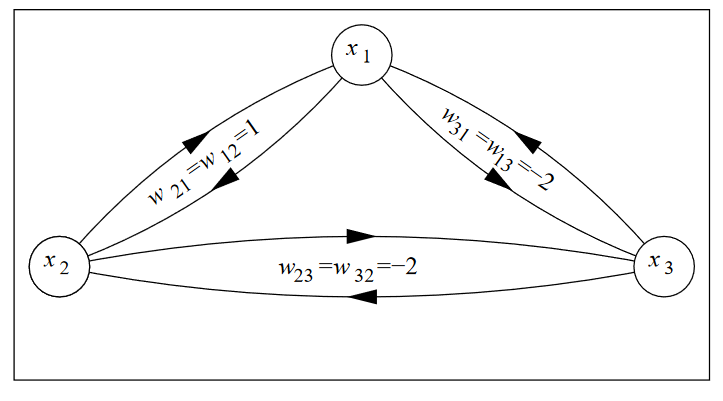
\includegraphics[width=\textwidth]{hopfieldnet}
            \caption{Hopfieldnet met drie neuronen.}
            
        \end{figure}
        \item De toestand wordt beschreven door de uitvoer van de drie neuronen als een binair getal te beschouwen. 
        \begin{itemize}
            \item Toestand $5 = (+ - +)$ waarbij $x_1$ en $x_3$ als uitvoer 1 hebben en $x_2$ uitvoer -1.
            \item Wat als we in deze toestand $x_2$ aanduiden voor herberekening.
            \item De invoer voor $x_2$ is $1 \cdot 1 - 2 \cdot 1 = -1$, zodat $x_2$ dezelfde uitvoer behoudt, en het net in toestand 5 blijft.
        \end{itemize}
        \item Er kan een transitietabel opgemaakt worden:
        \begin{table}[ht]
            \centering
            \begin{tabular}{| l | c  c  c |}
                \hline
                toestand & \multicolumn{3}{c|}{aangewezen neuron} \\
                \hline
                & $x_1$ & $x_2$ & $x_3$ \\
                \hline
                $0=(---)$ & 4 & 2 & 1 \\
                $1=(--+)$ & 1 & 1 & 1 \\
                $2=(-+-)$ & 6 & 2 & 3 \\
                $3=(-++)$ & 3 & 1 & 3 \\
                $4=(+--)$ & 4 & 6 & 5 \\
                $5=(+-+)$ & 1 & 5 & 5 \\
                $6=(++-)$ & 6 & 6 & 6 \\
                $7=(+++)$ & 3 & 5 & 6 \\
                \hline
            \end{tabular}
        \end{table}
        \item Toestand 6 en 1 zijn stabiel. Elke andere toestand zal ooit in toestand 1 of 6 komen door willekeurig neuronen aan te duiden.
        \begin{figure}[ht]
            \centering
            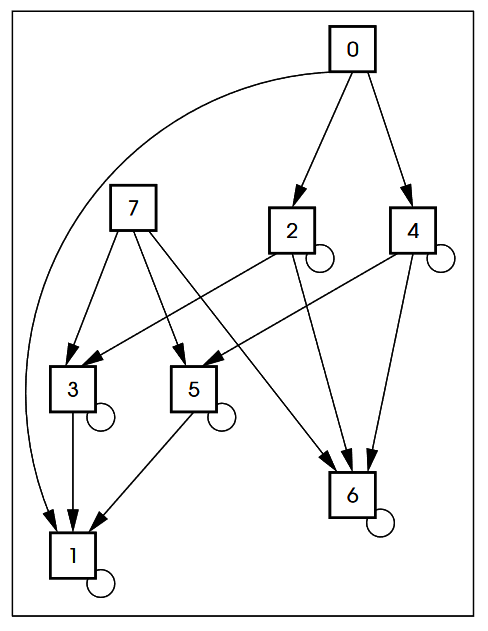
\includegraphics[width=0.5\textwidth]{overgangsdiagram}
            \caption{Overgangsdiagram van het netwerk.}
            
        \end{figure}
        \item Toestand 6 en 1 komen overeen met de twee patronen die het netwerk heeft opgeslagen. Bij een begintoestand (willekeurig bitpatroon van 3 bits) zal het netwerk evulueren naar één van deze twee toestanden, en wel diegene dat er het best op lijkt.
    \end{itemize}
\end{itemize}
\subsection{Algemene Hopfieldnetten}
\begin{itemize}
    \item Vorig voorbeeld was heel klein, stel nu een groter netwerk, met bijvoorbeeld duizend neuronen ($= 2^{1000}$ toestanden).
    \item De \textbf{energie} van een netwerk met $n$ neuronen wordt gedefinieerd als:
    $$E = -\frac{1}{2}\sum_{i=1}^{n}\sum_{j=1}^{n} \omega_{ij}u_iu_j$$ 
    \begin{itemize}
        \item Het product $u_iu_j$ is altijd gelijk aan $\pm 1$.
        \item Als $w_{ij}$ positief is, dan probeert de verbinding ervoor te zorgen dat $u_i$ en $u_j$ hetzelfde teken krijgen. Hoe groter de waarde $w_{ij}$, hoe meer het resultaat als 'vreemd' beschouwd wordt.
        \item Als $w_{ij}$ negatief is, dan is alles omgekeerd.
    \end{itemize}
    \item De energie van een net is een maat voor hoe vreemd de toestand is van het net.
    \item Duidt een neuron $x_k$ aan voor herberekening. \textbf{Twee} mogelijkheden:
    \begin{enumerate}
        \item De waarde van het neuron blijft hetzelfde zodat de toestand en energie behouden blijft.
        \item De waarde van het neuron verandert. Wat is nu de invloed hiervan op de energie van het netwerk?
        \begin{align*}
          E & = -\frac{1}{2}\sum_{i \neq k}^{n}\sum_{j \neq k}^{n} \omega_{ij}u_iu_j  -\frac{1}{2}\sum_{j} \omega_{kj}u_ku_j   -\frac{1}{2}\sum_{i} \omega_{ik}u_iu_k  \\
            & = -\frac{1}{2}\sum_{i \neq k}^{n}\sum_{j \neq k}^{n} \omega_{ij}u_iu_j -u_k\sum_{i \neq k}w_{ik}u_i
        \end{align*}
        \item De verandering van energieniveau is dan:

    \end{enumerate}
\end{itemize}
\section{Leren bij Hopfieldnetten}
\begin{itemize}
    \item Via de regel van Hebb.
    \item Als we de kans willen vergroten dat een bepaald patroon $U = (u_1, ..., u_n)$ als uitvoer voorkomt, dan moet de energie van dit patroon vermindert worden. 
    \begin{itemize}
        \item Dit komt neer met het veranderen van de gewichten in de richting van de uitvoeren:
        $$w_{ij} \rightarrow w_{ij} + u_iu_j \; \hbox{voor}\; i \neq j$$
        \item De wijziging in energie:
        \begin{align*}
            E_{nieuw}(U) & = -\frac{1}{2}\sum_{i=1}^{n}\sum_{j=1}^{n} (\omega_{ij} + \Delta\omega_{ij})u_iu_j \\
                         & = E_{oud}(U) -\frac{1}{2}\sum_{i=1}^{n}\sum_{j=1}^{n} \Delta\omega_{ij}u_iu_j  \\
                         & = E_{oud}(U) -\frac{1}{2}\sum_{i=1}^{n}\sum_{j=1}^{n} 1 \\
                         & = E_{oud}(U) - \frac{n^2 - n}{2}
        \end{align*}
    \end{itemize}
    \item Voor een ander patroon $V = (v_1, ..., v_n)$ die $k$ bits verschilt van $U$ daalt de energie ook:
    \begin{itemize}
        \item \begin{align*}
            E_{nieuw}(V) & = -\frac{1}{2}\sum_{i=1}^{n}\sum_{j=1}^{n} (\omega_{ij} + \Delta\omega_{ij})v_iv_j \\
                         & = E_{oud}(V) -\frac{1}{2}\sum_{i=1}^{n}\sum_{j=1}^{n} \Delta\omega_{ij}v_iv_j  \\
        \end{align*}
        en
        \begin{figure}[ht]
            \centering
            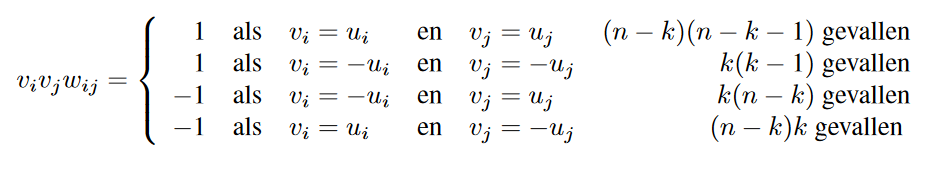
\includegraphics[width=\textwidth]{energy}
        \end{figure}

        dus
        $$E_{nieuw}(V) = E_{oud}(V) - \frac{(2k - n)^2 - n}{2} \\$$
    \end{itemize}

\end{itemize}

\section{Associatieve groepering}
\begin{itemize}
    \item Het komt bijna nooit voor dat dezelfde invoer herhaalde malen voorkomt in het leerproces.
    \item De stabiele eindtoestanden zijn een soort gemiddelde van groepen invoertoestanden die bij elkaar horen.
    \item Hopfieldnetten kunnen dan gebruikt worden om te classificeren zonder supervisie.
    \item Het algoritme:
    \begin{enumerate}
        \item Zet alle gewichten van het associatief geheugen op nul.
        \item Train het associatief geheugen op de gebruikelijke wijze met de gehele verzameling van punten.
        \item Houdt nu de gewichten van het associatief geheugen vast en presenteer weer alle punten. Punten die dezelfde uitvoer geven worden in dezelfde groep gestoken.
    \end{enumerate}
    \item In een andere versie wordt bij stap 3 dezelfde invoer meerdere malen gepresenteerd, maar worden verschillende neuronen gekozen om te herberekenen.
    \begin{itemize}
        \item Een punt dat meerdere uitvoeren heeft, wordt als grenspunt beschouwd.
        \item Als twee groepen meer grenspunten gemeen hebben dan een bepaald opgegeven getal, worden ze samengevoegd.
        \item Dit komt nauw overeen met transitiviteit.
    \end{itemize}
    \item Nog een alternatief: \textbf{winner-takes-all} netwerk:
    \begin{itemize}
        \item Neem $n$ analoge neuronen met uitvoerwaarden tussen $0$ en $1$ zodat het omringende netwerk ervoor zorgt dat de activatie van de neuron een functie is van de waarschijnlijkheid van elk van de alternatieven.
        \item Alle $n$ neuronen zijn nu onderling verbonden met negatieve gewichten.
    \end{itemize}
\end{itemize}

\section{Patroonvervollediging}
\begin{itemize}
    \item 
\end{itemize}